\begin{figure}[t]
    \centering
    % 4K
    \begin{subfigure}{\textwidth}
        \centering
        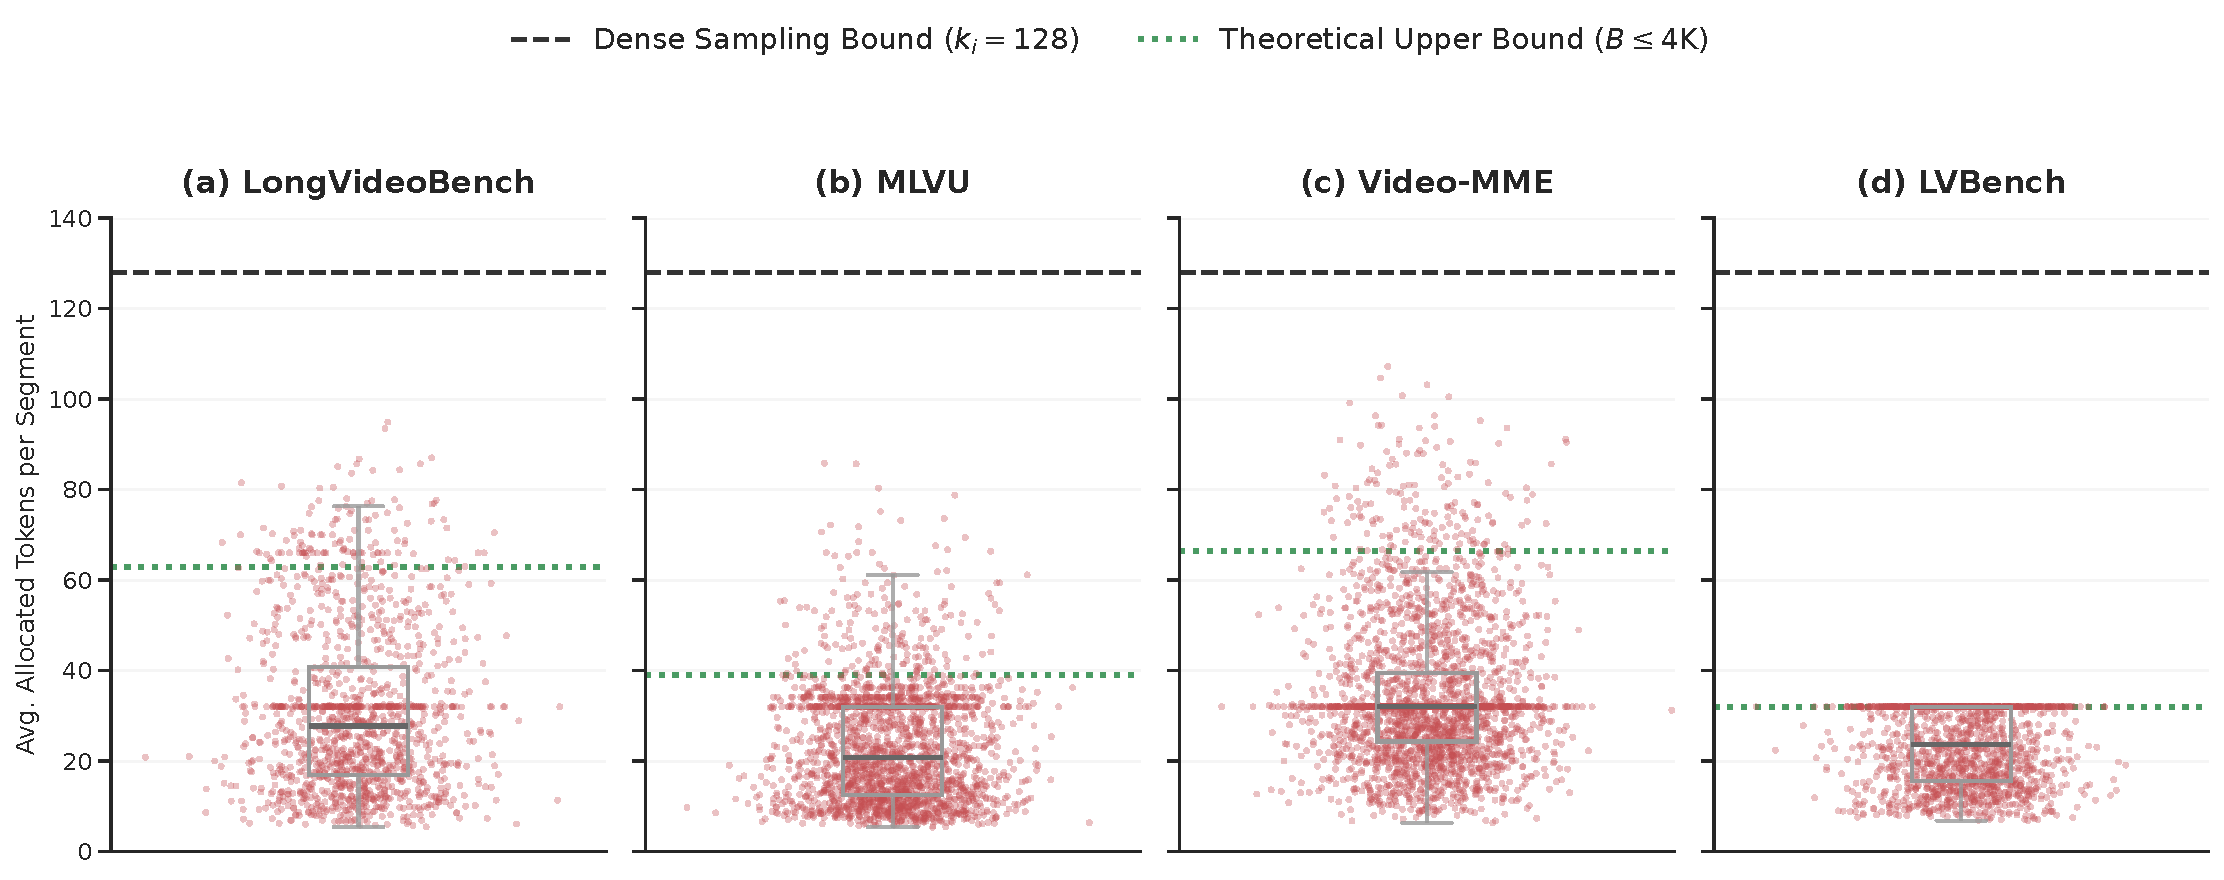
\includegraphics[width=0.95\linewidth]{supp/fig/token_consumption_rigorous_4k.pdf}
        \vspace{-0.5em}
    \end{subfigure}
    \\ \vspace{1em}
    % 8K
    \begin{subfigure}{\textwidth}
        \centering
        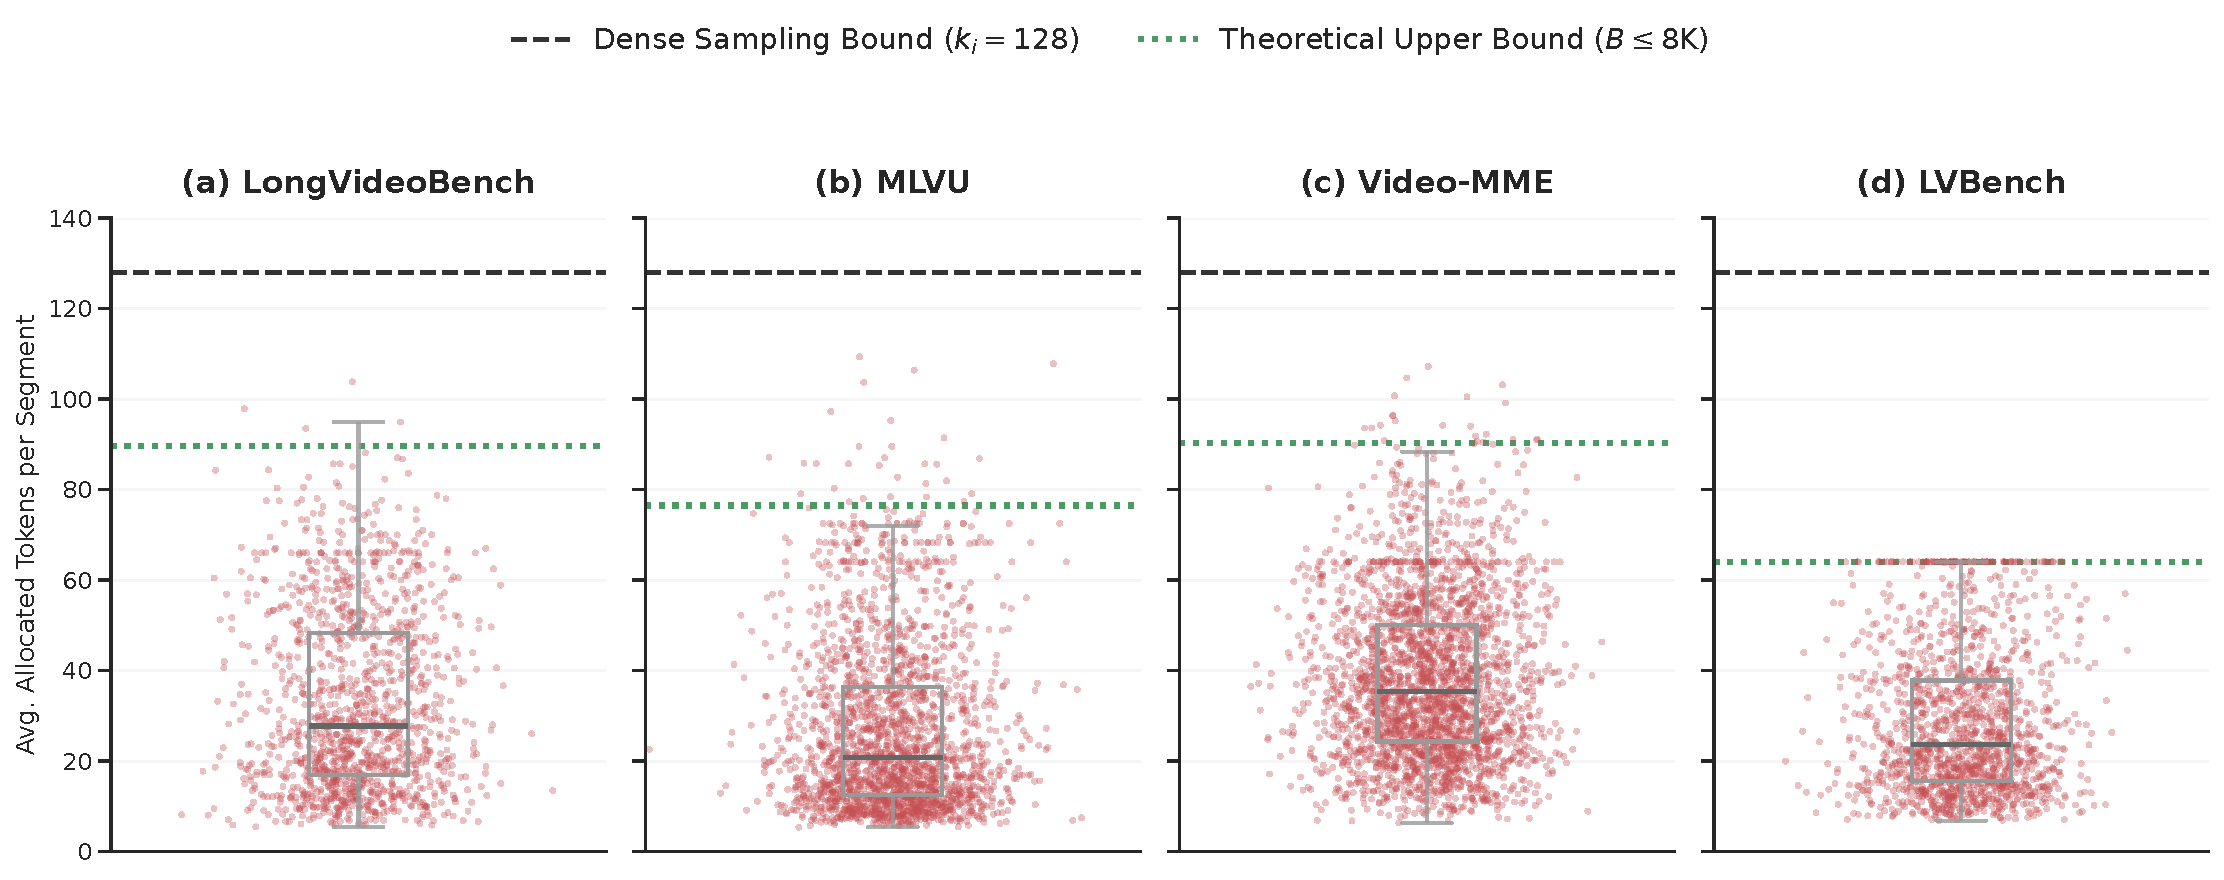
\includegraphics[width=0.95\linewidth]{supp/fig/token_consumption_rigorous_8k.pdf}
        \vspace{-0.5em}
    \end{subfigure}
    \caption{
        \textbf{Macro-level budget utilization and adaptation efficiency.}
        \textbf{(Top)} 4K budget; \textbf{(Bottom)} 8K budget.
        Each red dot denotes the \emph{average token consumption per segment} for a video sample. The dashed green line indicates the \emph{dataset-level average theoretical capacity}. Points above the line correspond to shorter videos whose per-segment capacity is higher than the dataset-wide average.
        \textbf{Adaptability:} On datasets with diverse video lengths (\eg, LongVideoBench, Video-MME), the consumption distribution remains well below the theoretical capacity, indicating query-driven compression.
        \textbf{Reliability:} On extremely long videos (LVBench), the token consumption forms a clear ceiling at the theoretical limit, demonstrating strict adherence to the global budget constraint.
    }
    \label{fig:macro_efficiency}
\end{figure}